\documentclass[aps,rmp,twocolumn,amsmath,amssymb,nofootinbib,superscriptaddress]{revtex4}

\newcommand{\bra}[1]{\langle#1|}
\newcommand{\ket}[1]{|#1\rangle}
\newcommand{\op}[2]{\hat{\textbf{#1}}_{#2}}
\newcommand{\dagop}[2]{\hat{\textbf{#1}}_{#2}^\dag}
\usepackage[pdftex]{graphicx}
\usepackage{mathrsfs}
\usepackage[colorlinks]{hyperref}
\usepackage[dvipsnames]{xcolor}

\newcommand{\sihui}[1]{{\color{Orchid}{#1}}}
\newcommand{\peter}[1]{{\color{YellowGreen}{#1}}}
\newcommand{\comment}[1]{{\color{blue}{#1}}}
\newcommand{\ah}{\hat{a}}
\newcommand{\adagh}{\hat{a}^\dag}

\begin{document}

\bibliographystyle{apsrev}

%
% Title
%

\title{The Resurgence of the Linear Optics Interferometer --- Recent Advances \& Applications}

%
% Authors
%

\author{Si-Hui Tan}
\email[]{sihui\_tan@sutd.edu.sg}
\affiliation{Singapore University of Technology and Design, 8 Somapah Road, Singapore}

\author{Peter P. Rohde}
\email[]{dr.rohde@gmail.com}
\homepage{http://www.peterrohde.org}
\affiliation{Centre for Quantum Software \& Information (CQSI), Faculty of Engineering \& Information Technology, University of Technology Sydney, NSW 2007, Australia}

\date{\today}

\frenchspacing

%
% Abstract
%

\begin{abstract}
\end{abstract}

\maketitle

\tableofcontents

\section{Introduction}

\sihui{Si-Hui can colour code things she adds like this}

\peter{And Peter can do it like this}

\comment{Let's add comments and questions like this}

Technical advancements have been made on many fronts. It is possible now to put single-photon sources and linear-optical networks on a silica chip. The advantage of using such integrated photonics over bulk optics is that it is more stable against phase fluctuations, and miniaturized. This increases the scalability of optical implementations of quantum information protocols.


\section{Mathematical background}
\comment{Mathematical representation for LO networks, and very basic background on quantum optics}\\

A idealized single photon in a quantum interferometer is described by its creation operator $\adagh_{j}$, where $j$ is the label of the mode the photon is in  within the interferometer. The creation and annihilation operators satisfy the bosonic comutator relationship $[\ah_{j},\adagh_{k}]=\delta_{j,k}$. A similar commutator relationship can be  written up when more degrees of freedom, such as polarization, orbital angular momentum, and time-bins \cite{bib:Tillmann2015,bib:Bozinovic2013, bib:Nicolas2014, bib:Humphreys2013, bib:Donohue2013}, are present. When multiple photons are present, they experience quantum interference when all quantum labels are the same.

The action of a $2d$-port linear optical interferometer (with an equal number of input and output ports) is expressed as an application of unitary operations on the creation operators,

\begin{align}
b_i^{\dag}=\sum_{j=1}^d U_{ij}a_j^\dag \ ,
\end{align}
where $a_j^\dag$ and $b_i^\dag$ are the creation operators of a single input and output photon in the $j$-th and $i$-th modes respectively, and $U\in SU(d)$. All such transformation can be expressed as sequence of beamsplitters and waveplates \cite{bib:Reck1994}. In the case when photons have additional labels, for instance, if they have internal labels on top of spatial labels, it is also possible to derive an analogous decomposition, known as a cosine-sine decomposition \cite{bib:Dhand2015}, that realizes the unitary transformation on the photons into a sequence of beamsplitters and internal transformations. Toolkits using group theory are being developed to deal with partial distinguishabilities among interfering photons \cite{bib:Tan2013,bib:deGuise2014,bib:deGuise2015}. Others use
quantum-to-classical transitions to explain multiparticle interference \cite{bib:Ra2013}. \sihui{Experimental implementation [Walmsley, Jennewein]}



\section{Optical encoding of quantum information on single-photons}

\section{Optical encoding of quantum information on single-photons}

Using quantum states of light, there are a multitude of approaches to encoding quantum information. Beginning with a logical qubit,
\begin{align}
\ket\psi_L = \alpha \ket{0}_L + \beta\ket{1}_L,
\end{align}
we now discuss the most prominent such encodings, which have been widely employed. We will specifically focus on single-photon encodings, as opposed to, for example, continuous variable encodings.

These encodings are all isomorphic to one another, but nonetheless, because they are represented using entirely different physical systems, they each exhibit their own unique advantages and disadvantages, and methods by which to implement operations upon them.

%\subsection{Single-photons}

\subsubsection{Polarisation}

In polarisation encoding, the polarisation of a single photon in a single spatial mode encodes a logical qubit. Specifically, we represent the logical qubit as,
\begin{align}
\ket\psi_L = \alpha\ket{H} + \beta\ket{V},	
\end{align}
where $H$ ($V$) denotes a horizontally (vertically) polarised single photon.

Polarisation encoding has the elegance that the most common optical error mechanisms, such as loss or path-length mismatch, affect the two logical basis states equally. Furthermore, single-qubit operations may be directly implemented using wave-plates, which implement a rotation in polarisation space. Relevant to the preparation of large entangled states, such as cluster states, polarising beamsplitters can be employed to perform non-deterministic Bell state projections.

When physically constructing protocols based on polarisation-encoding, for obvious reasons it is extremely important that optical components be polarisation-preserving. Not doing so would obviously corrupt the logical state. Some waveguide technologies, for example, exhibit different refractive indices for the two polarisations.

\subsubsection{Dual-rail}

In dual-rail encoding, a single photon encodes a logical qubit as a superposition across two spatial modes,
\begin{align}
\ket\psi_L = \alpha\ket{1,0} + \beta\ket{0,1},
\end{align}
where $\ket{i,j}$ is a two-mode state with $i$ ($j$) photons in the first (second) spatial mode. Using this encoding, phase-shifters and beamsplitters between the two spatial modes implement arbitrary single-qubit operations. Unfortunately, because the two basis states evolve via independent paths, our dual-rail qubits are susceptible to path-length-mismatch, a problem that does not affect polarisation encoding.

Converting between polarisation- and dual-rail-encoding is trivial using polarising beamsplitters, which separate horizontal and vertical components into distinct spatial modes, or vice-versa.

\subsubsection{Time-bins}

Time-bin qubits encode quantum information into the time-of-arrival of single photons, which have fixed polarisation and reside in a single spatial mode. Effectively, we discretise the direction of propagation of photons into discrete bins, which are treated as orthogonal basis states. Specifically, we are employing the encoding,
\begin{align}
\ket\psi_L = \alpha\ket{1}_{t}\ket{0}_{t+\tau} + \beta \ket{0}_{t}\ket{1}_{t+\tau},
\end{align}
where $\ket{0}_t$ ($\ket{1}_t$) denotes the vacuum (single-photon) state with arrival time $t$. Here $\tau$ is the time-bin separation, which must be sufficiently large that the temporal envelopes of neighbouring photons do not overlap, thereby ensuring orthogonality of the logical basis states.

This encoding is particularly resource-savvy, since a single spatial mode (e.g length of optical fibre) can encapsulate many time-bin qubits as a `time-bin-train'. The amount of quantum information that can be encoded into the train is limited only by its physical length.

Unlike polarisation or dual-rail encoding, time-bin encoding does not lend itself to `native' single-qubit operations. Rather, fast switching can be used to spatially separate neighbouring time-bins, implement a beamsplitter operation between them, before converting back to time-bin encoding.

\textbf{Need to edit the above together with what follows...}

It was first conceived for a single-photon passing through a Mach-Zedner interferometer with its two paths having different lengths \cite{bib:Brendel99}. If the photon passes through the shorter (longer) path, then it will arrive at the output port in an ``early" (``late") time bin labelled $\ket{e}$ ($\ket{\ell}$). Thus, photon will exit the interferometer in a state that is a superposition of these two states. Owing to difficulties in implementing qubit operations in this basis, it was at that time mostly used for demonstrating quantum communication over long distance \cite{bib:Thew02,bib:Marcikic04}. With the advent of faster optical components, and single-photon detectors, it has become feasible to perform any single qubit operations, and a post-selected CPHASE gate on time-bin qubits \cite{bib:Humphreys2013}. These gates form an universal set for quantum computing. At the same time, an ultrafast measurement technique for recovering time-bin qubits was also demonstrated \cite{bib:Donohue2013}.

In Humphrey {\it et al.} \cite{bib:Humphreys2013}, the time-bin qubits have a polarization register which is used to toggle between the mode in which qubits are stored and transmitted, {\it i.e.} the ``register" mode, and the mode in which qubits are manipulated, {\it i.e.} the ``processing" mode using a polarization rotation. Other operations needed are a displacement operation moves a time-bin qubit in the processing polarization in time relative to other qubits, a partial polarization rotation between the register and processing polarizations to couple them, and a photon number measurement in a bin. The polarization rotation and polarization coupling operations were implemented using a fast integrated optical switch based on polarization-sensitive cross-phase modulation with a switching time of less than 10 ps. The displacement was implemented using a calcite crystal of a size that is of a path-length difference equal to an integer multiple of the time-bin separation. Using these operations and post-selection using a single-photon detectors, the authors were able to perform a heralded CPHASE gate \cite{bib:KLM01}.

In Donohue {\it et al.} \cite{bib:Donohue2013}, time bins were converted into frequency bins using a nonlinear optical process known as sum-frequency generation (SFG) by pumping them on a crystal with a laser beam. The waveforms of the input photons and the pump beam are chirped in opposite directions in frequency, so that the output is a set of two peaks separated in frequency by an amount proportional to the time separation of the time bins. The output can then be measured with detectors that are slow compared to this separation. This is unlike conventional time-bin measurements which involves sending a time-bin state through an unbalanced Mach-Zedner interferometer matched to a bin separation to produce three output pulses that are separated by the time delay, and then having to resolve the middle pulse in time. 

Apart from these promising advances in produce time-bin qubit gates and ultrafast time-bin measurements, scalable networks using time-bin encoding are also possible using a loop-based architecture \cite{bib:Motes14}. This is discussed in more detail in Section \ref{sec:timebins}.

%\subsection{Continuous-variables}

%\subsubsection{Coherent states}

%\subsubsection{Squeezed states}

\section{Efficient circuit decompositions of linear optics networks}

The task of implementing an arbitrary quantum computation on linear optics comes down to implementing an arbitrary $n\times n$ unitary matrix. If a non-unitary transformation is desired, it can be embedded within a unitary matrix with larger dimensions. An algorithm for expressing an arbitrary unitary matrix {\it exactly} in terms of a sequence of $\mathcal{O}(n^2)$ beamsplitters and phase-shifters exists \cite{bib:Reck1994}. Alternatively, Mach-Zedner interferometer can also be used as building blocks instead of beamsplitters and phase shifters \cite{bib:Reck1994, bib:Englert2001}. Later, it has been shown that any nontrivial beam splitter, that does more than swapping modes around or add phases to them, is universal for linear optics \cite{bib:Bouland2014}. However, they do not provide a construction for arbitrary unitaries.

If the linear optical transformations can be realized on various degrees of freedom of light, then it is possible to realize a $n\times n$ arbitrary unitary transformation, where $n=n_s n_p$ for $n_s$ spatial modes, and $n_p$ internal modes, by a sequence of $\mathcal{O}(n_s^2 n_p)$ beamsplitters and $\mathcal{O}(n_s^2)$ internal transformations \cite{bib:Dhand2015}. Their approach reduces the required number of beamsplitters but increases the total number of optical elements needed increases by a factor of 2.

\section{Reconstructing the linear optical network}

In many practical situations, the structure of a linear optical device in terms of its constituent beamsplitters and phase shifters is known once it is built. However, owing to manufacturing imperfections, a precise characterization of these devices is still needed post-production. One of the ways, this can be done is via a quantum process tomography \cite{bib:Mitchell03,bib:Obrien04,bib:Lobino08,bib:Saleh11} . However, quantum process tomography is an expensive method in terms of number of measurements required to characterize the network, and it becomes impractical for large optical networks which can now be as large as 900 modes (check citations for number of modes). Alternative characterization protocols have been developed using quantum interference of various quantum light sources \cite{bib:Laing12,bib:Rahimi-Keshari13} in the linear optical device.

Generally, the unitary matrix of the $d\times d$ linear optical device are complex numbers $U_{ij}=r_{ij}e^{i\theta_{ij}}$, where $0 \leq r_{ij}\leq 1$, and $0\leq \theta_{ij}\leq 2\pi$. The scheme in \cite{bib:Laing12} relies on injecting one-photon and two-photon states into the linear optical network with correlated photon detection. First, they note some equivalencies: two unitaries $U$ and $U'$ are equivalent if there exist two diagonal unitary matrices $D_1^U$ and $D_2^U$ such that $U'=D^U_1 U D^U_2$, because these diagonal matrices are regarded as unknown and trivial phases on the input and output ports of the network, to which the one-photon and two-photon data are insensitive to. This reduces the first row and first column elements to real numbers, i.e. $\theta_{1j}=\theta_{i1}=0$. Second, the photon statistics remain unchanged under the complex conjugation of $U$. Thus, the imaginary part of $M_{2,2}$ must be non-negative. Then assuming that the first two rows and columns are non-vanishing, and that there is no total loss in the interferometer, the matrix to be recovered is
\begin{align}
U=\left (\begin{array}{cccc}
r_{11} & r_{12} & \ldots & r_{1m} \\
r_{21} & r_{22}e^{i\theta_{22}} &\ldots & r_{2m}e^{i\theta_{2m}}\\
\vdots & \vdots & \ddots & \vdots \\
r_{m1} & r_{m2}e^{i\theta_{m2}} & \ldots & r_{mm}e^{i\theta_{mm}}
 \end{array}\right ) \ .
\end{align}
In the paper, they showed that it is possible to write the paramaters $r_{ij}$, and $\theta_{ij}$ for $i,j\geq 2$ in terms of the $2m-1$ real parameters of the first column and row, and the visibility of two-photon inputs. The remaining $2m-1$ real parameters can be found via one-photon 
transmissions.  An increased accuracy of the characterization is possible by estimating and correcting systematic errors that arise due to mode mismatch \cite{Dhand16}. Others have used numerical methods to find the closest parameters that yield the observed visibilities \cite{bib:Spagnolo16,bib:Tillmann16}.

Another characterization method was presented that is similar to \cite{bib:Laing12} with the important exception that coherent states are to be used instead \cite{bib:Rahimi-Keshari13,bib:Heilmann15}. Such states are produced by a standard laser source, thus reducing the resource needed. The $r_{jk}$ terms are found by the square root of the ratios of output intensity at the $k$th port to the input intensity at the $j$th port. The remaining phases $\theta_{ij}$ are found by the interference pattern given by a two-mode coherent state $\ket{\alpha_1}\ket{\alpha_2}$ created by splitting a single coherent state on a 50-50 beamsplitter, and then imparting a relative phase, $\phi$, between them. The states $\ket{\alpha_1}$ and $\ket{\alpha_2}$ are input into port 1, and $j$ respectively. The output intensity at the $j$th port is 
\begin{align}
I_k=I(r_{1k}^2+r_{jk}^2+2 r_{1k}r_{kj}\cos(\phi+\theta_{jk})) \ ,
\end{align}
where $\theta_{jk}=0$ for $k=1$. By scanning the phase shift $\phi$ and then locating the maximum value of $I_k$ for $j=2,\ldots, m$, all unknown phases can be found via $\theta_{jk}=2\pi-\phi$. An elegant extension of the scheme of Rahimi-Keshari {\it et al.} removes the need for precise control of the phase shift $\phi$ \cite{bib:Heilmann15} by suggesting instead to plot the output intensity $I_k$ with respect to the input intensity $I$. In time, the natural drift in the laser source will cause this plot to trace out an ellipse, known as a Lissajous figure. whose orientation and direction of evolution will give the phase $\theta_{jk}$ and its sign respectively.

\section{Experimental implementation}

\subsection{State preparation}

\subsubsection{Single-photons}

Sources of single photons for applications of quantum information processing are 
separated into two main categories \cite{bib:Kok05}; those produced by spontaneous 
parametric down-conversion (SPDC), and those by solid-state emitters in a cavity. 
Both categories have seen some leaps recently in their record production of numbers 
of single photons while preserving good qualities in their single photons. To 
date, SPDC has been able to produce up to ten entangled photons 
\cite{bib:WangChen16,bib:Chen17}, and five-photon quantum interference has been 
reported using a quantum dot emitter in a microcavity \cite{bib:WangHe16}.

In SPDC, a nonlinear crystal with a large $\chi^{(2)}$ is pumped with a strong 
laser and with a small probability, the pump beam is absorbed by the crystal to 
produce two beams of lower energy known as the signal and idler beams. Owing to 
conservation of energy and momentum, the two beams have spatio-temporal 
correlations that can be engineered to produce twin-beam states which have 
perfectly correlated photon numbers. If a single photon were to be detected in one 
of the beams, and then it is certain that the other beam would be in the state of a 
single photon. Some commonly used nonlinear crystals for SPDC are beta barium 
borate (BBO), periodically poled lithium niobate (PPLN), and periodically poled 
potassium titanyl phosphate (PPKTP). Recently, techniques using bismuth triborate 
(BiBO) have improved to the extent of becoming one of the record-holders of single-
photon production \cite{bib:WangChen16}.



Solid-state single photon sources come from semiconducting nanostructures and 
nitrogen valencies (NV) centers in diamond. Both types are versatile and efficient 
sources of single photons, however, the photons they produce have suffered from 
lack of indistinguishability that is necessary for quantum information processing.
Recent developments in the former show promising developments. Notably, much 
progress has been made using resonant excitation of quantum dots. Laser pulses are 
used to excite their electronic resonance and trigger the emission of single 
photons \cite{bib:Muller07,bib:Vamivakas09, bib:Flagg09,bib:Ates09, bib:Dirk10,
bib:1748,bib:Jayakumar13,bib:Wei14,bib:Muller14,bib:Unsleber15,
bib:237403,bib:Sweeney14}. An architecture that embeds the quantum dot in a 
micropillar cavity with the same resonant frequency as the dot exploits the 
Purcell effect to achieve higher single-photon production efficiency 
†\cite{bib:Ding16,bib:213601}. 
Such resonant excitation of quantum dots overcome the homogenous broadening of the 
excited state that causes degradation of photon purity and hence improves
indistinguishability. Using a time-bin loop-based architecture \cite{bib:Motes14} 
on a stream of single photons produced by such a quantum dot, the same group was 
able to demonstrate quantum interference between five indistinguishable photons 
\cite{bib:WangChen16}.



\subsubsection{Einstein-Podolsky-Rosen (EPR) pairs}

\sihui{ Discuss producing Bell pairs using SPDC, and transforming them into GHZ and cluster states.}

An EPR pair is a pair of qubits that are in a Bell state together, that is, one of the following states: $\{\ket{0}_A\ket{0}_B\pm\ket{1}_A\ket{1}_B,\{\ket{1}_A\ket{0}_B\pm\ket{1}_A\ket{0}_B\}$. Such a pair of qubits forms the simplest example of entangled states, and its production from spontaneous parametric down-conversion (SPDC) have been the mainstay of entanglement source for quantum optical processing \cite{bib:Kim01,bib:Kim03,bib:Brida07,bib:Dayan07}. In some applications, it may be desired to have the EPR pairs conditionally prepared, {\it i.e.} successfully prepared only under certain measurement outcomes of auxiliary modes. Some theoretical proposals have been proposed \cite{bib:Pittman03,bib:Sliwa03,bib:Walther07}, and in some cases demonstrated \cite{bib:Wagenknecht10,bib:Barz10}.

\subsubsection{Greenberger-Horne-Zeilinger (GHZ) states}

\subsubsection{Cluster states}

\subsection{Linear optics networks}

\subsubsection{Bulk-optics}

\subsubsection{Waveguides}

\subsubsection{Time-bins}\label{sec:timebins}

\cite{bib:Motes14}

Using time-bin encoding of optical qubits, the obvious question is how to perform operations upon them. In \cite{bib:Motes14}, a dual-loop architecture was presented for implementing arbitrary passive linear-optics on photonic pulse-trains, shown in Fig.~\ref{fig:FL_arch}.

\begin{figure}[!htb]
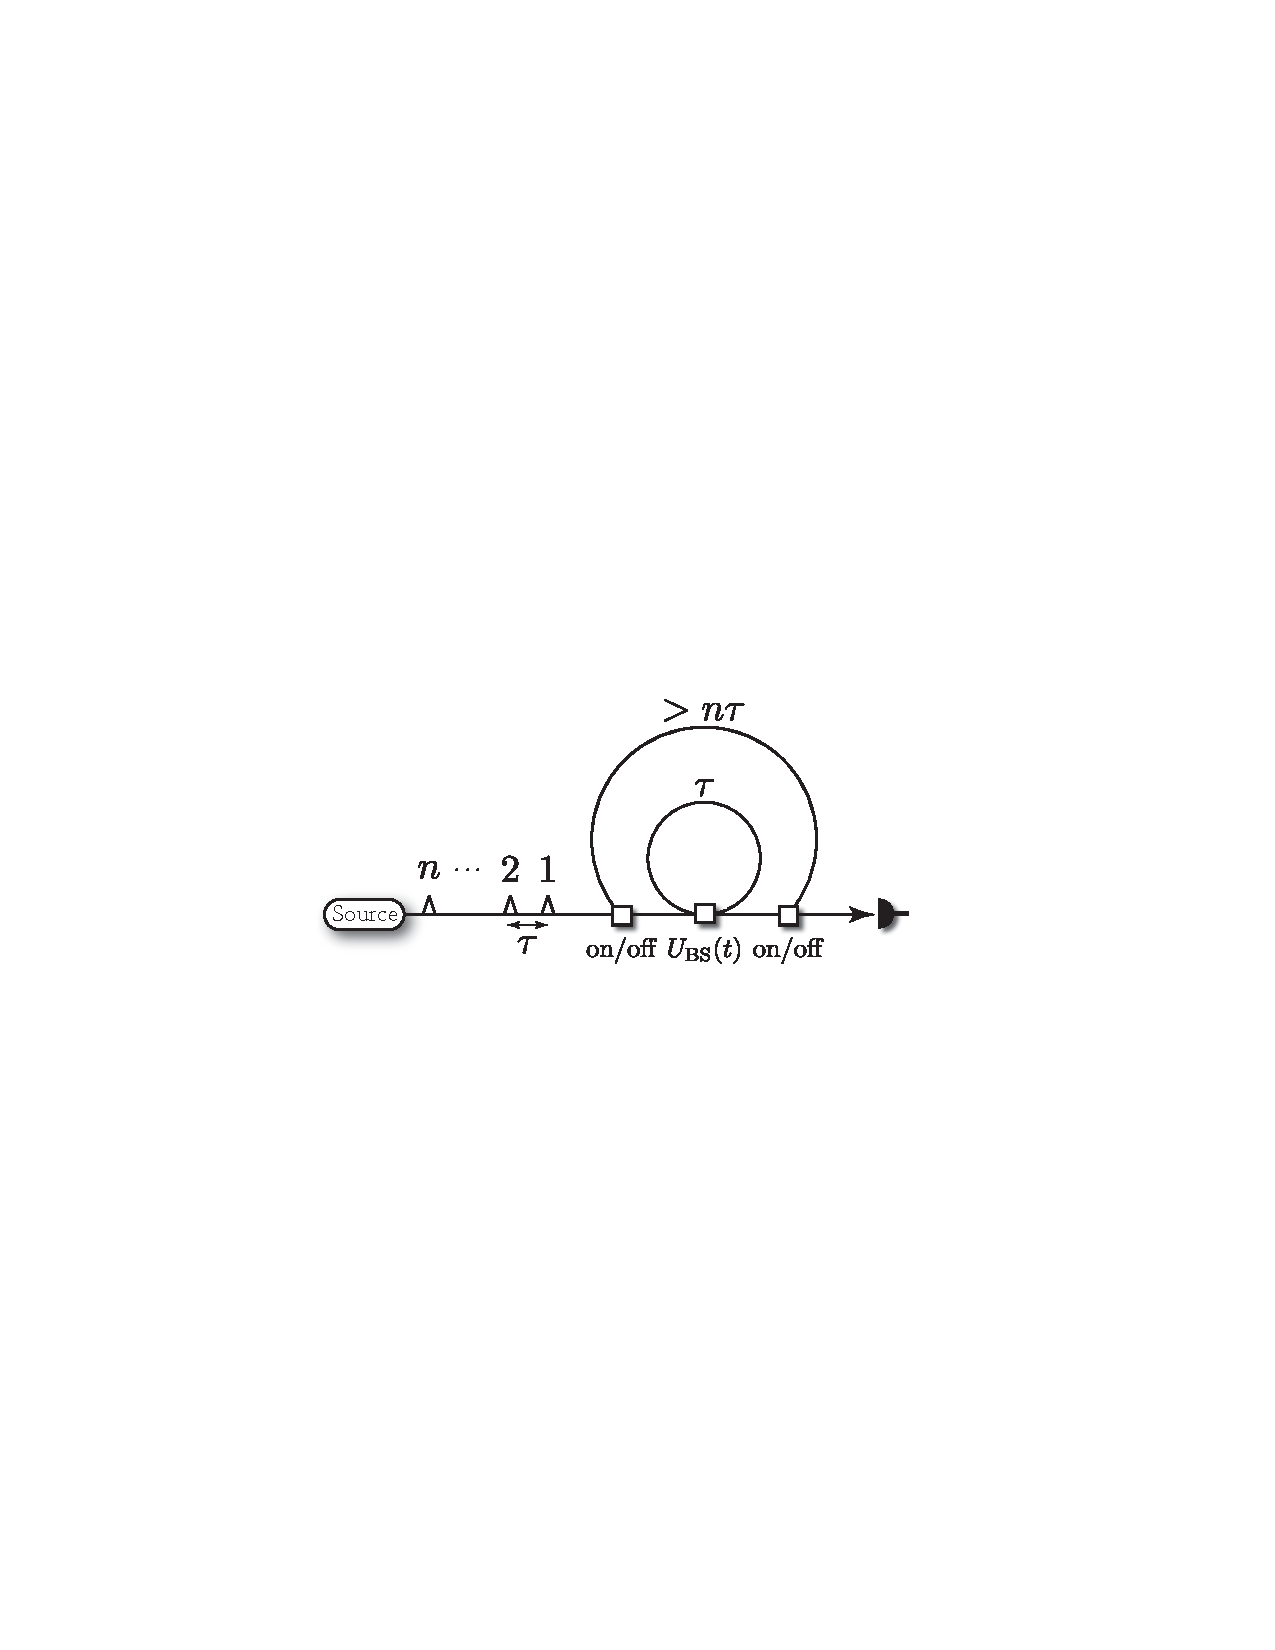
\includegraphics[width=\columnwidth]{full_architecture}
\caption{A fibre-loop architecture for implementing arbitrary linear optics operations upon a time-bin-encoded pulse-train. The source prepares the temporally encoded pulse-train, with time-bin separation $\tau$. The pulse-train then enters a dual-loop configuration. The inner loop has length exactly $\tau$, while the outer one has length $>n\tau$ ($n$ is the number of optical modes). The architecture is controlled via three dynamically controlled beamsplitters. The first and last need only be on/off switches, whose sole purpose is to couple in the prepared pulse-train, keep it within the outer loop for the required duration, and then couple out of the outer loop, yielding the transformed pulse-train. The central beamsplitter must be able to implement arbitrary classically-controlled beamsplitter operations.} \label{fig:FL_arch}	
\end{figure}

The architecture is frugal in its use of optical components, requiring only three dynamic beamsplitters, and several lengths of fibre. The beauty of this architecture is that the experimental requirements do not increase with the number of optical modes. The only parameter that scales with the number of optical modes is the outer loop, which must be at least long enough to house the entire time-bin-encoded pulse-train. Note, however, that the central beamsplitter must be controllable at sub-$\tau$ time-scales, so as to enable each temporal mode to be addressed individually, which is technically challenging.

The workings of the scheme can be thought of as follows: the inner loop allows arbitrary beamsplitter operations between neighbouring time-bins; the outer loop does nothing interferometric, but rather enables the pulse-train to undergo as many applications of the inner loops as necessary. It then follows that this scheme is universal for linear optics, as a sufficient number of beamsplitter operations between neighbouring modes enables universal decompositions, such as that by \cite{Reck}.

As a simple example of how such time-bin encoding maps to other encodings, in Fig.~\ref{fig:PBS_TB} we show the isomorphism between the polarising beamsplitter operation and a pairwise temporal beamsplitter operation.

\begin{figure}[!htb]
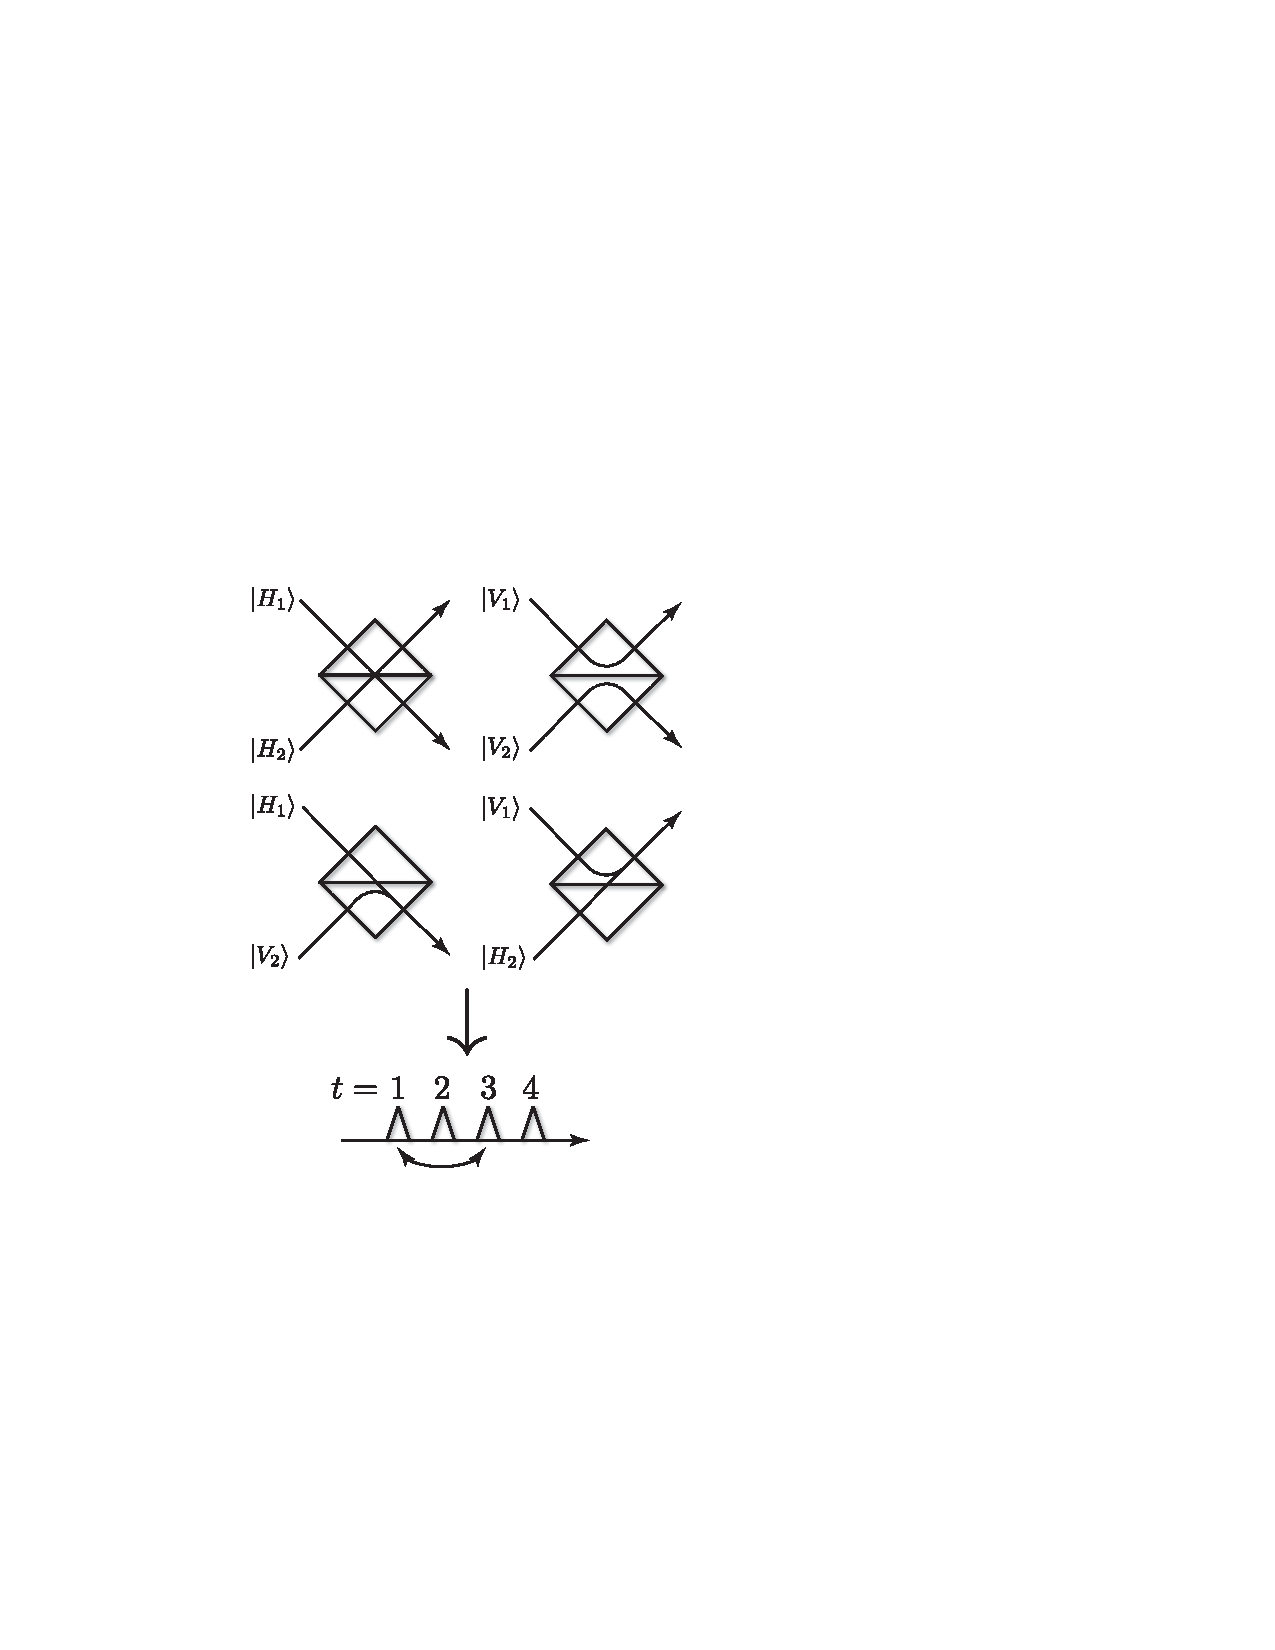
\includegraphics[width=0.7\columnwidth]{PBS_TB}
\caption{Mapping between two polarisation-encoded qubits undergoing a polarising beamsplitter (PBS) operation, and its equivalent representation using 4 time-bins in a pulse-train. The PBS completely reflects (transmits) the vertical (horizontal) polarisations. The evolution of the four logical basis states, and their respective outputs, are shown explicitly. Writing out this PBS transformation in matrix form yields a permutation. Taking this permutation and relabelling the modes, we obtain the time-bin transformation shown underneath -- a simple swap of two of the four time-bins.} \label{fig:PBS_TB}	
\end{figure}

The above description applies to passive linear optics, which is sufficient for protocols such as {\sc BosonSampling}, but insufficient for universal optical quantum computation, which requires the addition of ancillary states, and measurement with fast-feedforward. To address this, it was shown in \cite{Rohde} that by dynamically preparing ancillary pulse-trains (from the already-existing source), classically controlled by time-resolved measurements at the output, and changing the switching sequence, we can effectively couple in and out arbitrary subsets of the optical modes, enabling partial measurements to be implemented.

\subsection{Measurement}

\subsubsection{Photodetection}

\comment{Discuss number-resolved and bucket detectors, multiplexed detection, APDs, current micropillar detectors}

\subsubsection{Homodyning}

\section{Applications for linear optics interferometry}

\subsection{Linear optics quantum computation}

\subsection{Boson-sampling}

\subsection{Quantum metrology}

\comment{Discuss NOON states - Heisenberg limited}

\comment{Discuss MORDOR scheme}

\subsection{Encrypted quantum computation}

\section{State of the art}

\comment{Discuss where experiments are at at the moment}

\section{Conclusion}

%
% Acknowledgments
%

\begin{acknowledgments}
P.P.R. is funded by an ARC Future Fellowship (project FT160100397).
\end{acknowledgments}

%
% Bibliography
%

\bibliography{paper}

\end{document}
